\documentclass{amsmlaj}

\begin{document}
\lecturesol{Homework 3}{Ke Tran}{m.k.tran@uva.nl}{April 26, 2016}
{Andrea Jemmett}{11162929}{andreajemmett@gmail.com}{N/A}

\begin{problem}
Consider the inference problem of evaluating $p(\vt{x}_n|\vt{x}_N)$ for the
graph shown in Figure \ref{fig:chain}, for all nodes $n \in \{1,\dotsc,N-1\}$.
Show that the message passing algorithm can be used to solve this efficiently,
and discuss which messages are modified and in what way.

\begin{figure}[H]
\begin{center}
\begin{tikzpicture}
\node[nObs,] (x1) at (0,0) {};
\node at (0,-0.5) {$x_1$};
\node[nObs,] (xn_1) at (3,0) {};
\node at (3,-0.5) {$x_{n-1}$};
\node[nObs,] (xn) at (4.5,0) {};
\node[nObs,] (xn1) at (6,0) {};
\node at (6,-0.5) {$x_{n+1}$};
\node at (4.5,-0.5) {$x_n$};
\draw [-, thick, red] (x1) -- (1,0);
\draw[dashed, thick, red] (1,0) -- (2,0);
\draw [-, thick, red]  (2,0) -- (xn_1);
\draw [-, thick, red]  (xn_1) -- (xn);
\draw [-, thick, red]  (xn) -- (xn1);
\draw [-, thick, red]  (xn1) -- (7,0);
\draw[dashed, thick, red] (7,0) -- (8,0);
\node[nObs,] (xN) at (9,0) {};
\node at (9,-0.5) {$x_N$};
\draw [-, thick, red] (8,0) -- (xN);
% draw messages
\node at (2,0.7) {$\mu_\alpha(x_{n-1})$};
\draw [->, thick, blue] (2,0.4) -- (2.5,0.4);
\node at (3.75,0.7) {$\mu_\alpha(x_n)$};
\draw [->, thick, blue] (3.5,0.4) -- (4,0.4);
\node at (5.25,0.7) {$\mu_\beta(x_n)$};
\node at (7,0.7) {$\mu_\beta(x_{n+1})$};
\draw [->, thick, blue] (5.5,0.4) -- (5,0.4);
\draw [->, thick, blue] (7,0.4) -- (6.5,0.4);
\end{tikzpicture}
\caption{Chain of nodes model}
\label{fig:chain}
\end{center}
\end{figure}
\end{problem}

\begin{problem}
Apply the sum-product algorithm to the chain of nodes model in Figure
\ref{fig:chain}  and show that the results of message passing algorithm are
recovered as a special case, that is
\begin{eqnarray}
p(x_n) & = & \frac{1}{Z}\mu_\alpha(x_n)\mu_\beta(x_n) \nonumber\\
\mu_\alpha(x_n) & = & \sum\limits_{x_n-1} \psi_{n-1,n}(x_{n-1},x_n)\mu_\alpha(x_{n-1}) \nonumber\\
\mu_\beta(x_n) & = & \sum\limits_{x_{n+1}} \psi_{n+1,n}(x_{n+1},x_n)\mu_\beta(x_{n+1}) \nonumber
\end{eqnarray}
where $\psi_{i,i+1}(x_i,x_{i+1})$ is a potential function defined over clique $\{x_i,x_{i+1}\}$.
\end{problem}


\begin{problem}
Run sum-product algorithm on the graph in Figure \ref{fig:simplegraph} with node
$x_3$ designed as the root. Using the computed messages given in \emph{p.409 Bishop}.
\begin{enumerate}
\item  Show that the correct marginals are obtained for $x_1$ and $x_3$.
\item Show that the sum-product algorithm on this graph gives the correct joint distribution for $x_1$, $x_2$.
\end{enumerate}

\begin{figure}[H]
\begin{center}
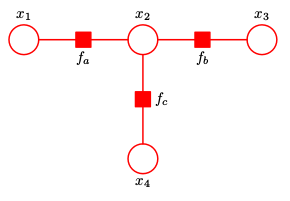
\includegraphics[width=.4\textwidth]{simplegraph.png}
\caption{A simple factor graph}
\label{fig:simplegraph}
\end{center}
\end{figure}

\end{problem}

\begin{problem}
Show that the marginal distribution for the variables $\vt{x}_s$ in a factor
$f_s(\vt{x}_s)$ in a tree-structured factor graph, after running the sum-product
message passing algorithm, can be written as
\[
p(\vt{x}_s) = f_s(\vt{x}_s) \prod\limits_{i \in \text{ne}(f_s)} \mu_{x_i \to f_s(x_i)}
\]
where ne($f_s$) denotes the set of variable nodes that are neighbors of the factor node $f_s$
\end{problem}

\end{document}

